\documentclass[12pt]{book}
\usepackage{fontspec}
\setmainfont{TeX Gyre Pagella}
\usepackage[paperwidth=8in,paperheight=8in,margin=0.6in]{geometry}
\usepackage{xcolor}
\usepackage{tikz}
\pagestyle{empty}
\setlength{\parindent}{0pt}

\newcommand{\artnote}[1]{{\color{gray!70}\small\itshape [Illustration: #1]}\par\vspace{0.3in}}
\newcommand{\bigline}[1]{{\Huge #1}\par}
\newcommand{\pagenum}[1]{\vfill{\color{gray!50}\footnotesize #1}}
\newcommand{\sprollpage}{\newpage\vspace*{0.4in}}

\begin{document}

% ============ FRONT COVER ============
\thispagestyle{empty}
\begin{center}
\vspace*{1.2in}
{\Huge \textbf{SPROLL 00}}\\[0.4in]
{\huge \textbf{A Difference}}\\[0.6in]

\begin{tikzpicture}
\filldraw[fill=black] (-0.5,0) circle (0.13in);
\draw[fill=orange!60] (0.3,-0.15) -- (0.5,0.25) -- (0.7,-0.15) -- cycle;
\end{tikzpicture}\\[0.6in]
{\large \textit{a book before the beginning}}\\[0.3in]
{\small The Sproll Curriculum $\cdot$ Cycle I: Pops}
\end{center}

% ============ PAGE 2: half-title / indicia ============
\sprollpage
\begin{center}
\vspace*{1.5in}
{\Large The Sproll Curriculum}\\[0.2in]
{\normalsize Cycle I --- Pops: Things, Differences, and Counting}\\[0.6in]
{\small Sproll 00 of 40}
\end{center}
\pagenum{2}

% ============ PAGE 3 ============
\sprollpage
\begin{center}
\vspace*{0.8in}
\artnote{a single small solid dot, alone in the center of an otherwise empty page}

\begin{tikzpicture}
\filldraw[fill=black] (0,0) circle (0.15in);
\end{tikzpicture}
\vspace{0.4in}
\bigline{Here is something.}
\end{center}
\pagenum{3}

% ============ PAGE 4 ============
\sprollpage
\begin{center}
\vspace*{0.8in}
\artnote{a small orange triangle, alone in the center of the page}

\begin{tikzpicture}
\draw[fill=orange!60] (-0.2,-0.15) -- (0,0.25) -- (0.2,-0.15) -- cycle;
\end{tikzpicture}
\vspace{0.4in}
\bigline{Here is something else.}
\end{center}
\pagenum{4}

% ============ PAGE 5 ============
\sprollpage
\begin{center}
\vspace*{0.6in}
\artnote{two hands mid-clap, simple line drawing, small motion marks between the palms}

\begin{tikzpicture}
\draw[line width=2pt] (-0.4,0) -- (-0.05,0.1);
\draw[line width=2pt] (0.4,0) -- (0.05,0.1);
\draw[line width=1pt] (0,0.15) -- (0,0.4);
\draw[line width=1pt] (-0.15,0.2) -- (-0.3,0.45);
\draw[line width=1pt] (0.15,0.2) -- (0.3,0.45);
\end{tikzpicture}
\vspace{0.4in}
\bigline{A loud clap is something.}
\end{center}
\pagenum{5}

% ============ PAGE 6 ============
\sprollpage
\begin{center}
\vspace*{0.6in}
\artnote{three faint concentric rings, drawn thin and light, suggesting a quiet sound}

\begin{tikzpicture}
\draw[line width=1pt, gray!60] (0,0) circle (0.25in);
\draw[line width=1pt, gray!60] (0,0) circle (0.42in);
\draw[line width=1pt, gray!60] (0,0) circle (0.58in);
\end{tikzpicture}
\vspace{0.4in}
\bigline{A quiet sound is something too.}
\end{center}
\pagenum{6}

% ============ PAGE 7 ============
\sprollpage
\begin{center}
\vspace*{0.6in}
\artnote{a soft gray shadow-shape on the ground, cast by an unseen object just off the page}

\begin{tikzpicture}
\filldraw[fill=gray!40, draw=none] plot [smooth cycle] coordinates
{(-0.4,-0.1) (-0.1,0.1) (0.3,0.05) (0.45,-0.2) (0.1,-0.3) (-0.3,-0.3)};
\end{tikzpicture}
\vspace{0.4in}
\bigline{A shadow is something too.}
\end{center}
\pagenum{7}

% ============ PAGE 8 ============
\sprollpage
\begin{center}
\vspace*{0.5in}
\artnote{a large, dense, tangled scribble filling most of the space, deliberately messy and complicated}

\begin{tikzpicture}
\draw[line width=2pt] plot [smooth, tension=1.2] coordinates
{(0,0) (0.3,0.4) (-0.2,0.6) (0.5,0.7) (0.1,0.2) (-0.4,0.5) (0.2,-0.3)
(-0.3,-0.5) (0.4,-0.4) (0,0.1) (-0.5,0.1) (0.3,-0.1) (0,-0.5) (0.5,-0.1)};
\end{tikzpicture}
\vspace{0.3in}
\bigline{A big, complicated scribble is something.}
\end{center}
\pagenum{8}

% ============ PAGE 9 ============
\sprollpage
\begin{center}
\vspace*{0.8in}
\artnote{a single tiny dot, much smaller than the one on the first page}

\begin{tikzpicture}
\filldraw[fill=black] (0,0) circle (0.04in);
\end{tikzpicture}
\vspace{0.4in}
\bigline{So is a tiny dot.}
\end{center}
\pagenum{9}

% ============ PAGE 10 ============
\sprollpage
\begin{center}
\vspace*{0.5in}
\artnote{no new image; small versions of the dot, clap, shadow, and scribble arranged in a loose row, all drawn at equal size}
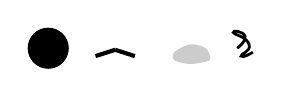
\begin{tikzpicture}
\filldraw[fill=black] (-1.5,0) circle (0.1in);
\draw[line width=1.5pt] (-0.9,-0.1) -- (-0.65,-0.02);
\draw[line width=1.5pt] (-0.4,-0.1) -- (-0.65,-0.02);
\filldraw[fill=gray!40, draw=none] plot [smooth cycle] coordinates
{(0.1,-0.05) (0.3,0.05) (0.5,0) (0.55,-0.15) (0.3,-0.2) (0.1,-0.15)};
\draw[line width=1pt] plot [smooth, tension=1.2] coordinates
{(0.9,0) (1.0,0.15) (0.85,0.2) (1.05,0.05) (0.95,-0.1) (1.1,-0.05)};
\end{tikzpicture}
\vspace{0.4in}
\bigline{Something does not mean big.}\vspace{0.1in}
\bigline{Something does not mean loud.}\vspace{0.1in}
\bigline{Something does not mean round.}\vspace{0.2in}
{\Huge \textbf{Something just means: here it is.}}
\end{center}
\pagenum{10}

% ============ PAGE 11 ============
\sprollpage
\begin{center}
\vspace*{0.7in}
\artnote{two identical small dots, side by side, same size, same color}

\begin{tikzpicture}
\filldraw[fill=black] (-0.4,0) circle (0.13in);
\filldraw[fill=black] (0.4,0) circle (0.13in);
\end{tikzpicture}
\vspace{0.4in}
\bigline{They look alike.}
\end{center}
\pagenum{11}

% ============ PAGE 12 ============
\sprollpage
\begin{center}
\vspace*{0.4in}
\artnote{two identical small dots, this time placed far apart -- one near the top left of the page, one near the bottom right}

\begin{tikzpicture}
\filldraw[fill=black] (-1.8,1.4) circle (0.13in);
\filldraw[fill=black] (1.8,-1.4) circle (0.13in);
\end{tikzpicture}
\vspace{2.2in}
\bigline{Are they the same?}
\end{center}
\pagenum{12}

% ============ PAGE 13 ============
\sprollpage
\begin{center}
\vspace*{0.5in}
\artnote{a large circular boundary containing a small busy scene inside it: a few dots, a triangle, a scribble mark, all clustered together, with the boundary drawn clearly around the whole group}
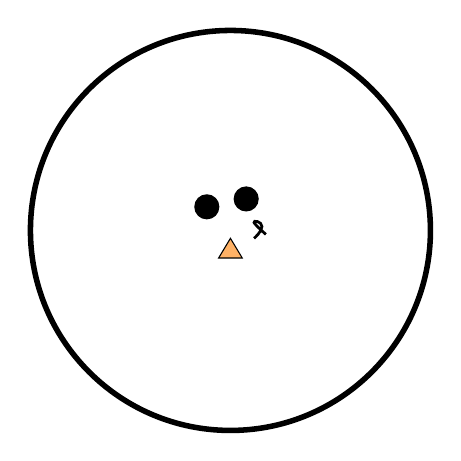
\begin{tikzpicture}
\draw[line width=2pt] (0,0) circle (1in);
\filldraw[fill=black] (-0.3,0.3) circle (0.06in);
\filldraw[fill=black] (0.2,0.4) circle (0.06in);
\draw[fill=orange!60] (-0.15,-0.35) -- (0,-0.1) -- (0.15,-0.35) -- cycle;
\draw[line width=1pt] plot [smooth, tension=1.2] coordinates
{(0.3,-0.1) (0.4,0.05) (0.3,0.1) (0.45,-0.05)};
\end{tikzpicture}
\vspace{0.3in}
\bigline{Can many things be treated as one?}
\end{center}
\pagenum{13}

% ============ PAGE 14 ============
\sprollpage
\begin{center}
\vspace*{0.5in}
\artnote{the same circular scene from the previous page, completely unchanged -- not merged, not resolved -- with a small, faint question mark drawn just beside the boundary}
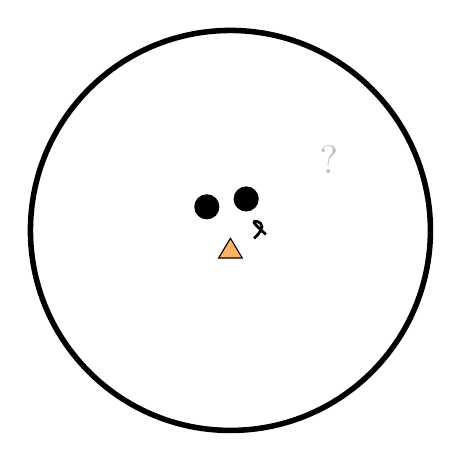
\begin{tikzpicture}
\draw[line width=2pt] (0,0) circle (1in);
\filldraw[fill=black] (-0.3,0.3) circle (0.06in);
\filldraw[fill=black] (0.2,0.4) circle (0.06in);
\draw[fill=orange!60] (-0.15,-0.35) -- (0,-0.1) -- (0.15,-0.35) -- cycle;
\draw[line width=1pt] plot [smooth, tension=1.2] coordinates
{(0.3,-0.1) (0.4,0.05) (0.3,0.1) (0.45,-0.05)};
\node[gray!50] at (1.25,0.9) {\Large ?};
\end{tikzpicture}
\vspace{0.3in}
\bigline{Sometimes.}\vspace{0.15in}
{\Large But what do we mean by ``one''?}
\end{center}
\pagenum{14}

% ============ PAGE 15 (closing / hand-off) ============
\sprollpage
\begin{center}
\vspace*{0.5in}
\artnote{three plain, unlabeled shapes evenly spaced with open room between them: a circle, a triangle, a square, none highlighted, none connected}
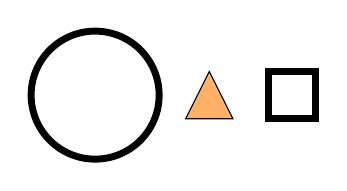
\begin{tikzpicture}
\draw[line width=2.5pt] (-1.3,0) circle (0.32in);
\draw[fill=orange!60] (-0.15,-0.3) -- (0.15,0.3) -- (0.45,-0.3) -- cycle;
\draw[line width=2.5pt] (0.9,-0.3) rectangle (1.5,0.3);
\end{tikzpicture}
\vspace{0.5in}
\bigline{Here are three things.}\vspace{0.2in}
{\Large Something could happen.}
\vspace{0.5in}\\
{\small \textit{--- turn the page for Sproll 01: Something Happened ---}}
\end{center}
\pagenum{15}

% ============ PAGE 16: Note for Grown-Ups (backmatter) ============
\sprollpage
\vspace*{0.3in}
{\large \textbf{A Note for Grown-Ups}}
\vspace{0.2in}

\normalsize
This book teaches no arithmetic and introduces no formal vocabulary. Its only goal is to let a child practice the single act underneath all of mathematics: noticing that something can be told apart from everything around it.

\vspace{0.15in}
On purpose, this book never uses the word ``Pop.'' Distinguishing something is a prerequisite for the mathematics that follows, but it is not yet the first formal move of that mathematics. Sproll 01 begins exactly where this book leaves off: when something happens to what could happen next.

\vspace{0.15in}
The two open questions in this book, ``Are they the same?'' and ``Can many things be treated as one?'', are not meant to be answered for the child. Sitting with them is the point. Later Sprolls, in particular Sproll 07, return to both questions with considerably more to say.

\vspace{0.3in}
{\small Sproll 01: Something Happened continues directly from this book's final page.}
\pagenum{16}

\end{document}
